\section{Problem Overview}
\label{sec:overview}

The scope of the problem can be thought of as follows: we aim to integrate data analytics within
a document in a manner that maximizes the ability of the reader to understand the core information
being presented. Existing solutions such as notebooks and literate programming are limited by their
labour-intensive nature, and the lack of interactivity between data visualizations and accompanying text.

This large scale problem is a difficult one, there are many sub-problems that do not have immediate answers.
Two of the main issues are scale and abstraction: modern data analysts employ complex models and large datasets.
Bridging the gap between -- for example -- the results of a regression analysis and the natural language description
of the results is difficult, due to the presence of steps like feature-selection. Furthermore with modern approaches
such as neural networks, the analytical methods themselves can become black-boxes.

Automating this process would require a system that can generate code which correctly performs the data analysis,
which is a task well beyond the scope of current research in AI. We shall instead restrict our attention to a smaller
problem, namely how do we link text and visualizations based on the results of a data analysis that has already been
performed. The larger problem should be considered a long-term goal for such a research program.

\subsection{Potential Users}
We envisage a wide range of use-cases that could make use of the sort of system we are proposing.
In all cases, the potential user is an author of a document, attemping to communicate some sort of information to a potential reader.
We have so far considered the following potential users:

\paragraph{Data Scientists:} data scientists already use tools like notebooks in order to package their results, and
communicate information. Our system could be used to build something that looks like a typical notebook interface, but
provides automated linking from the cells containing text to the cells containing visualizations. The idea of self-certifying
text is useful in this context, since it would allow another data scientist to interrogate assumptions made in the analysis,
which is a boon to reproducibility.

\paragraph{Science journalists:} a science journalist would benefit from being able to write articles using our tool.
Since their readers may not necessarily be experts in the topic they are trying to communicate, augmenting visualizations
with interactivity allows a layperson to better understand the concept being communicated. An broadly educated reader
will also benefit from the ability to understand assumptions made when writing the article.

\paragraph{Educators:} a great deal of education and self-study is now done through online resources, such as blogs.
These resources, whilst undoubtedly useful, miss a key part of in-person education, which is the ability for a student
to ask questions of the teacher. Whilst our system will in no way attempt emulate a teacher, the ability for a student
to interact with the document and to understand the data dependencies induced by the code. Self-certifying text could
allow the reader to gain a better understanding of the meaning of subject specific language used in the document. 

\subsection{Linking Text To Visual and Data Objects}
We shall make the assumption that the author of an article has already written the code which performs
their data analysis, and the code which turns the results into useful visualisations. Restricting the scope to the problem of
automatically generating code which references the pre-computed visual and data objects.
Indeed, without having solved this more restricted problem it is difficult to see how one would approach
the more general problem of embedding data analytics directly into text.

\subsection{The Linguistic Sorts of Linked Text}
We begin by breaking down the sorts of linked text that the developer may
be interested in generating. 

\begin{figure}
   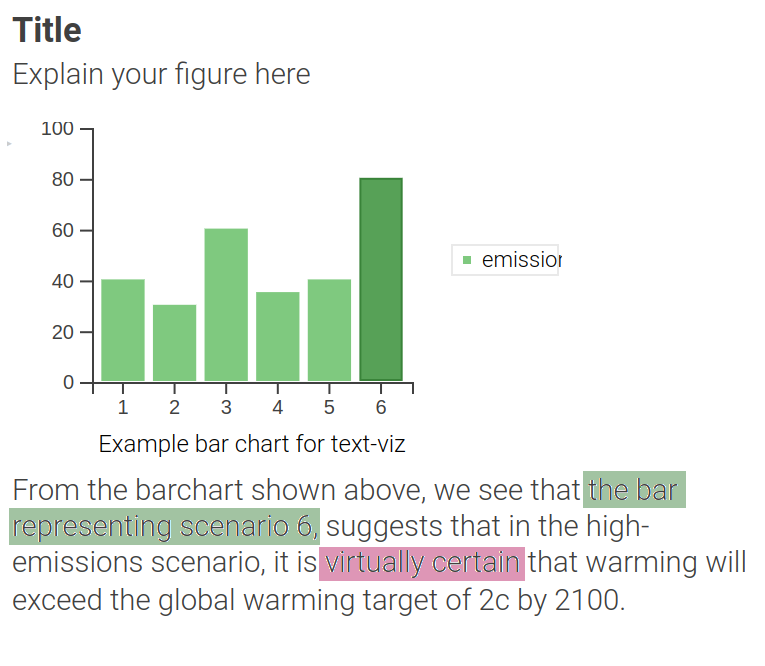
\includegraphics[width=0.7\textwidth]{fig/text-viz-types.png}
   \caption{Two sorts of linked text}
   \label{fig:linked-text-types}
\end{figure}

\subsubsection{Graded Adjectives}
A graded adjective is an adjective that can be modified to make its form stronger or weaker.
As an example, consider mapping ranges of probabilities onto natural language. If the probability
of an event occurring is $1$, we can say it is \emph{certain} to occur. If instead it is $0.99$
or some other value arbitrarily close to $1$, we will \emph{grade} the adjective to weaken it:
it is \emph{virtually certain} to occur. In \figref{linked-text-types}, this corresponds to the text
highlighted in pink.

Considered in more depth, we arrive at the concept of modalities in natural language. Similar to 
the concepts in modal logic, a modality allows the expression of concepts such as necessity or possibility.
In the context described above, the idea that a probability is \emph{virtually certain} introduces the modality of
possibility -- an event must be possible in order to be virtually certain to occur. Even something simple
like the discussion of probabilities above can combine the two into the idea of graded modality:
if something is ``very likely'', we would still believe that it is less likely to occur than something that
is ``virtually certain''. Handling these sorts of linguistic constructs will be a key part of addressing
the problem. 

\subsubsection{Selecting Visual Elements: Iteration, Scope and Mereology}
Text that refers to objects of discourse is relatively common, but even direct references are non-trivial 
linguistically. \figref{linked-text-types} shows a figure taken from a report summarizing recent climate 
science for policymakers. Even this simple example shows the complexity of the problem: the text highlighted
in orange refers to the collection of bar-charts shown on the left hand side, introducing a set of 5 bar-charts
into the scope of discourse. The text highlighted in green refers to the bars within these charts, mapping 
a narrowing of scope across the bar-charts that have already been introduced. Then, the text highlighted in
purple narrows this scope further to talk about the bar representing total warming, again within each of the
charts at the same time. 

This illustrative example showcases several sub-problems our system will need to be able to handle. First
is that of creating an iterative scope for the references that follow. We can imagine that the orange-highlighted
text effectively creates an iterable, which the green highlighted text maps over. The purple-highlighted text
then maps over the iterable created by the green highlighted text. This sort of iteration is a common feature of natural language,
and any well-designed system should allow for such expressions to be written by the author, and linked appropriately.

In order to reference substructures that appear within the 5 charts, the system must be able to walk arbitrarily 
into structured data objects. In linguistics this is referred to as ``mereology'', the study of relationships
between parts and wholes. In our case, one could imagine the collection of 5 charts as the whole, with each
individual bar-chart being a part of that whole. Because all 5 charts are structurally the same (of the same type),
we can apply the same walk to each of them: bar-charts in our language have a field called \kw{bars}, a list
of the various bars. In this light, we can imagine the green-highlighted text as walking into the \kw{bars} field
of the charts, and the purple-highlighted text as walking into this list, and selecting the bar with the label "total warming".

Automatically generating sentences that refer to visual elements in this way is one of the core problems we aim to solve.

\begin{figure}
   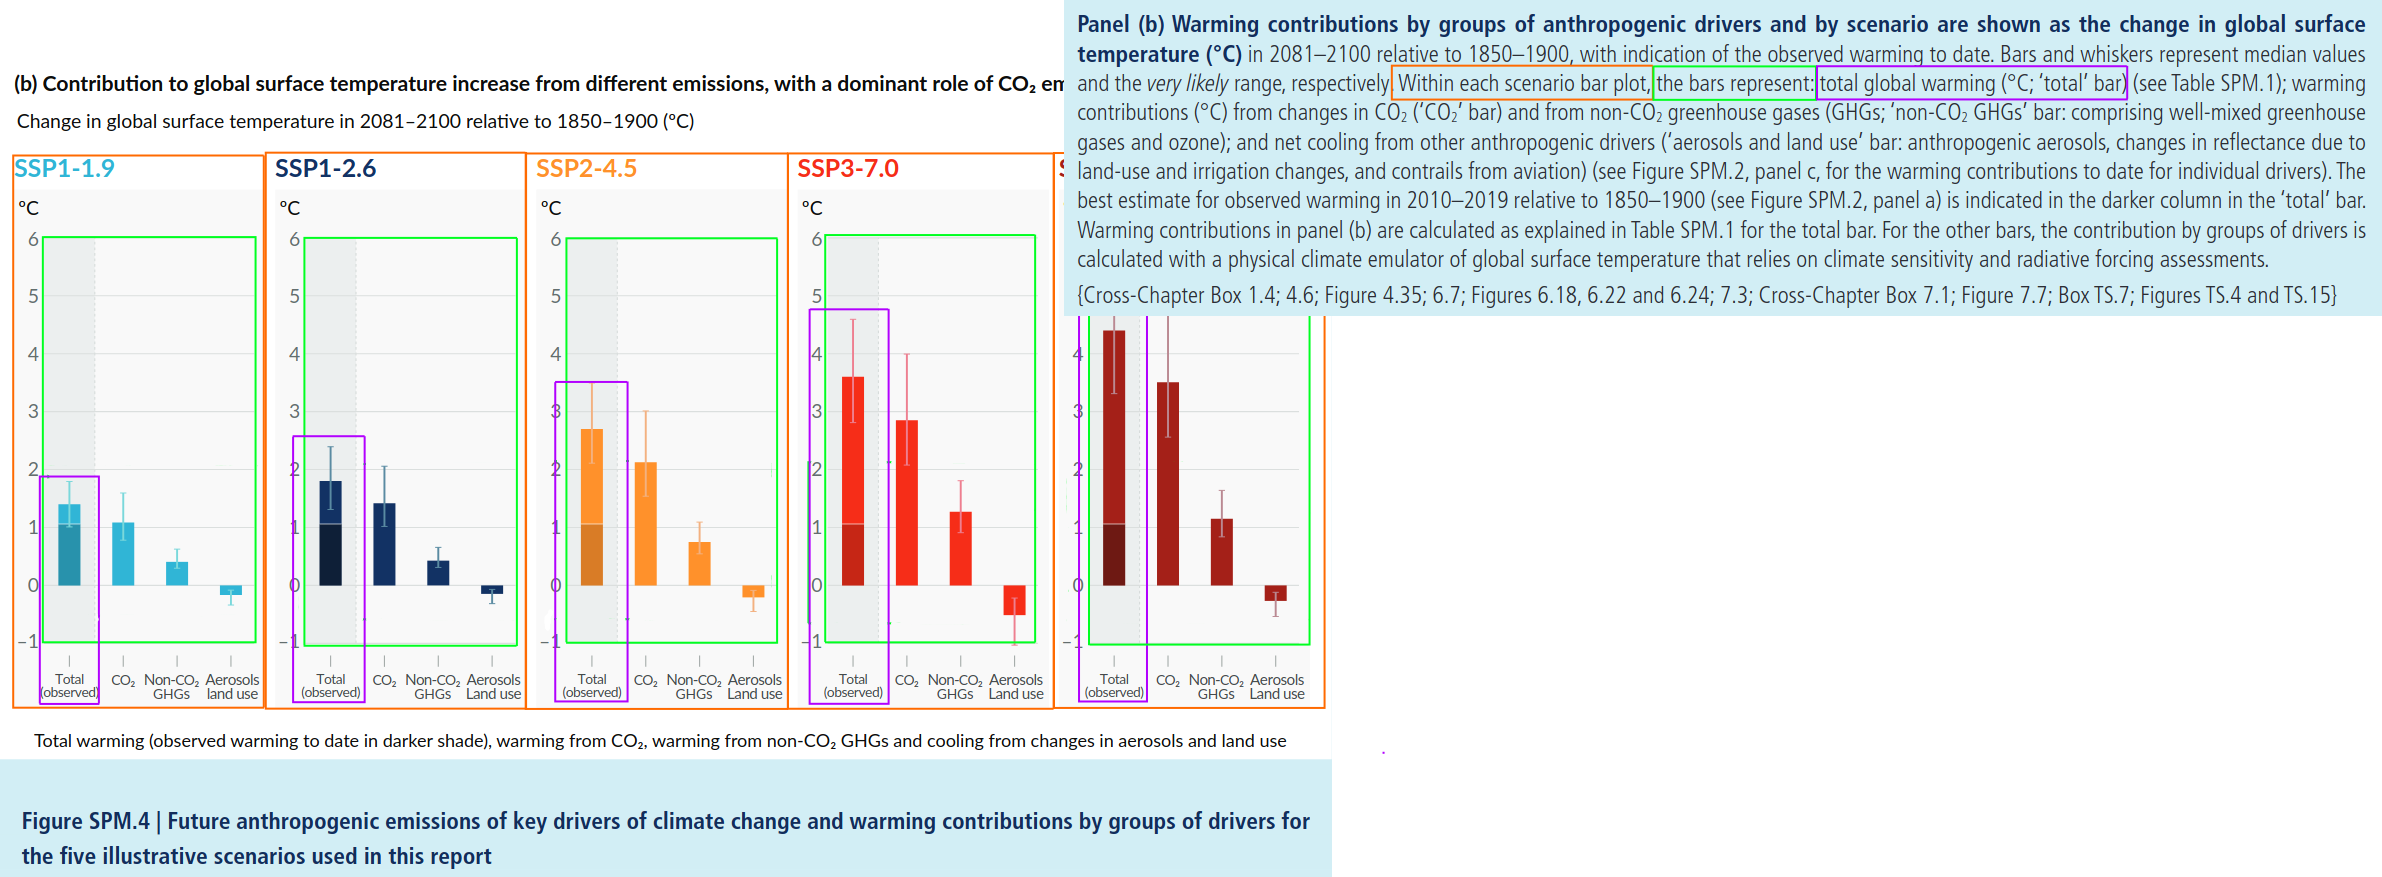
\includegraphics[width=0.9\textwidth]{fig/ipcc-visual-elements.png}
   \caption{Examples of scope in linked text}
   \label{fig:visual-element-scope}
\end{figure}

\subsubsection{Quantitative Expressions}
On its surface, directly embedding a quantitative expression into the text seems to be the simplest
of the linguistic categories we have identified thus far, but this may not be the case. Embedding
a percentage may be simple: requiring the user to only provide a numerical value, and scaling it
to be in the range of $0$-$100$, but more complicated expressions, such as a description of a calculation
may be more difficult to synthesize. 

\subsection{Challenges}
Applying language models to the task of code generation is not new, however the aim of generating code that
itself produces natural language appears to be a novel one. We currently anticipate the following challenges,
and will add more as the work progresses.

\paragraph{Small number of examples:} as a language, Fluid is incredibly niche, and so we have a very small corpus
of programs on which to train a language model. Further, we currently only have 2 example programs that actually make
use of the \kw{LinkedText} construct which we intend to use. The problem then is how to best make use of the capabalities
of current language models in this context. For example, should we perform some sort of few-shot learning or prompt-engineering
technique on a large pre-trained model, should we augment our corpus of training examples manually or both? If we take a meta-learning
perspective (\todo{CITE}), we may run into problems of the model preferring syntax and function names from the languages we use to
train the model.

\paragraph{Counter-intuitive dependency relation:} at the moment, dependencies that are computed by Fluid can be counter-intuitive.
Until we revamp the underlying dependency model, we will need to generate code that follows the pattern of ``consuming'' input
data in order to produce the output text. This may be a problem for things like generating direct references to visual elements.

\paragraph{Potentially complex code:} for many purposes, we want to store the data objects being referred to in variables. This 
could mean complicated code, and cluttering a source file. We will potentially need to find a general pattern for this sort of thing,
so that an authors document doesn't get filled with extraneous variable declarations. 